Note that each period is independent, and therefore separation decisions only depends $z$ in the period. Let separation decision be represented by $s(z) \in \{0,1\}$.\\

\subsection*{Part 1}

Under given condition
\begin{equation*}
    s(z) = \begin{cases}
        1 ~~~\text{if}~ z \ge \hat z\\
        0 ~~~\text{if}~ z < \hat z
    \end{cases}
\end{equation*}

The value of a job for the firm is
\begin{align*}
    J(z) = z - w(z) + \beta \mathbb E\left[ \max\{J(z'), V-\xi\}    \right]
\end{align*}

The value of vacancy is 
\begin{align*}
    V = c  + \beta \mathbb E[q(\theta) \max\{J(z'), V-\xi\}  + (1-q(\theta))V]
\end{align*}

The value of an employed worker is 
\begin{align*}
    E(z) = w(z) + \beta \mathbb E[ \max\{E(z'), U\}]
\end{align*}

The value of an unemployed worker is 
\begin{align*}
    U = b + \beta \mathbb E[ (1-f(\theta))U(z') + f(\theta) \max\{E(z'), U\}]
\end{align*}


\subsection*{Part 2}

Due to free entry, $V = 0$. We have 
\begin{align*}
    S(z) &= E(z) + J(z) - U - (V-\xi)    \\
    &= z -b + (1-\beta) \xi + \beta \mathbb E \left[ \max\{J(z')+\xi, 0\} + (1-f(\theta))\max\{E(z')-U, 0\} \right]\\
    &= z -b + (1-\beta) \xi + \beta \mathbb E \left[ \max\{J(z')+\xi, 0\} +  \max\{E(z')-U, 0\} - f(\theta)\max\{E(z')-U, 0\} \right]
\end{align*}

Note that $s(z) = 0 \iff J(z')+\xi\ge 0, E(z')-U \ge 0$.\\ Therefore, $\max\{J(z')+\xi, 0\} +  \max\{E(z')-U, 0\} = \max\{J(z')+\xi + E(z')-U, 0\} = \max\{S(z'), 0\}$. Hence, 

\begin{align*}
    S(z) &= z -b + (1-\beta) \xi + \beta \mathbb E \left[ \max\{S(z'), 0\} - f(\theta)\max\{E(z')-U, 0\} \right]\\
    &= z -b + (1-\beta) \xi + \beta \int_{\hat z}^\infty S(\tilde z)dG(\tilde z) - \beta f(\theta) \int_{\hat z}^\infty (E(\tilde z) - U)dG(\tilde z) \tag{1-1}
\end{align*}

\subsection*{Part 3}
For any $z>z'$, the firm and worker accepts the match and generate surplus $S(z)$. From the expression above, $S'(z) = 1$. For $z=z'$, the firm and worker are indifferent between separating and working. Therefore, the surplus must be zero. Otherwise, is surplus was positive, they would accept the match and split the surplus. Hence
$$ S(z) = z - \hat z$$

\subsection*{Part 4}

Nash bargaining problem
\begin{align*}
    w(z) &= \operatorname{argmax}_{\{E(z) - U, J(z) + \xi\}} (E(z) - U)^{\gamma}(J(z) + \xi)^{1-\gamma}\\
        &~~ s.t.~~ S(z) = z-\hat z = E(z) - U + J(z) + \xi
\end{align*}

which is equivalent to 
\begin{align*}
    w(z) &= \operatorname{argmax}_{\{E(z) - U, J(z) + \xi\}} \gamma \log (E(z) - U) + (1-\gamma)\log (J(z) + \xi)\\
        &~~ s.t.~~ S(z) = z-\hat z = E(z) - U + J(z) + \xi
\end{align*}

Using lagrnage multiplies $\lambda$, the first order conditions are given by 
\begin{align*}
    \gamma \frac{1}{E(z) - U} &= \lambda \\
    (1-\gamma) \frac{1}{J(z) + \xi} &= \lambda \\
\end{align*}

Using $S(z) = E(z) - U + J(z) + \xi = \frac{1}{\lambda} $, we have 

\begin{align*}
    E(z) - U &= \gamma S(z)\\    
    J(z) + \xi &= (1-\gamma) S(z)
\end{align*}

\subsection*{Part 5}
Substituting $E(z) - U = \gamma S(z)$ in equation 1-1, and setting $S(\hat z) = 0$, we get

\begin{align*}
    0 &= \hat z -b + (1-\beta) \xi + \beta (1-\gamma f(\theta)) \int_{\hat z}^\infty (\tilde z-\hat z)dG(\tilde z) \tag{1-6}
\end{align*}

we can rewrite this as 

\begin{align*}
    f(\theta) = \frac{\hat z -b + (1-\beta) \xi}{\gamma\beta \int_{\hat z}^\infty (\tilde z-\hat z)dG(\tilde z)}+ \frac{1}{\gamma}
\end{align*}

If $\hat z$ increases, then the integral value decreases and therefore $f(\theta)$ increases. This gives a positive relationship. An increase in vacancies or decrease in unemployment increases the job finding rate for workers, and therefore workers demand a higher wage that increases the cut-off productivity $\hat z$. 

\subsection*{Part 6}

As described in part 1, we have the value of vacancy 
\begin{align*}
    V = c  + \beta \mathbb E[q(\theta) \max\{J(z'), V-\xi\}  + (1-q(\theta))V]
\end{align*}

Setting $V=0$, this gives 
\begin{align*}
    c &= \beta q(\theta) \mathbb E[\max\{J(z') + \xi, 0\} - \xi]\\
    &= \beta q(\theta) \mathbb E[(1-\gamma)\max\{S(z')\} - \xi]\\
    &= \beta q(\theta) \left((1-\gamma)\int_{\hat z}^\infty (\tilde z-\hat z)dG(\tilde z) - \xi\right) \tag{1-7}
\end{align*}

An increase in $\hat z$ decreases the intgral, and therefore requires a higher value of $q(\theta)$. Since $q$ is a decreasing function of $\theta$, this defines a decreasing relationship between $\theta$ and $\hat z$. An increase in vacancies or decrease in unemployment results in a lower worker finding rate of firms, and therefore firms are willing to accept matches with lower productivity.

\subsection*{Part 7}

Equation (1-6) implies a increasing relationship between $\hat z$ and $\theta$ due to workers demand for higher surplus when markets become tighter. Equation (1-7) shows a decreasing relationship between $\hat z$ and $\theta$ due to firms accepting a lower productivity workers as markets become tighter. Since both these equations hold in equilibrium, the solutions is given by the intersection.

\subsection*{Part 8}

\begin{figure}[H]
  \centering
  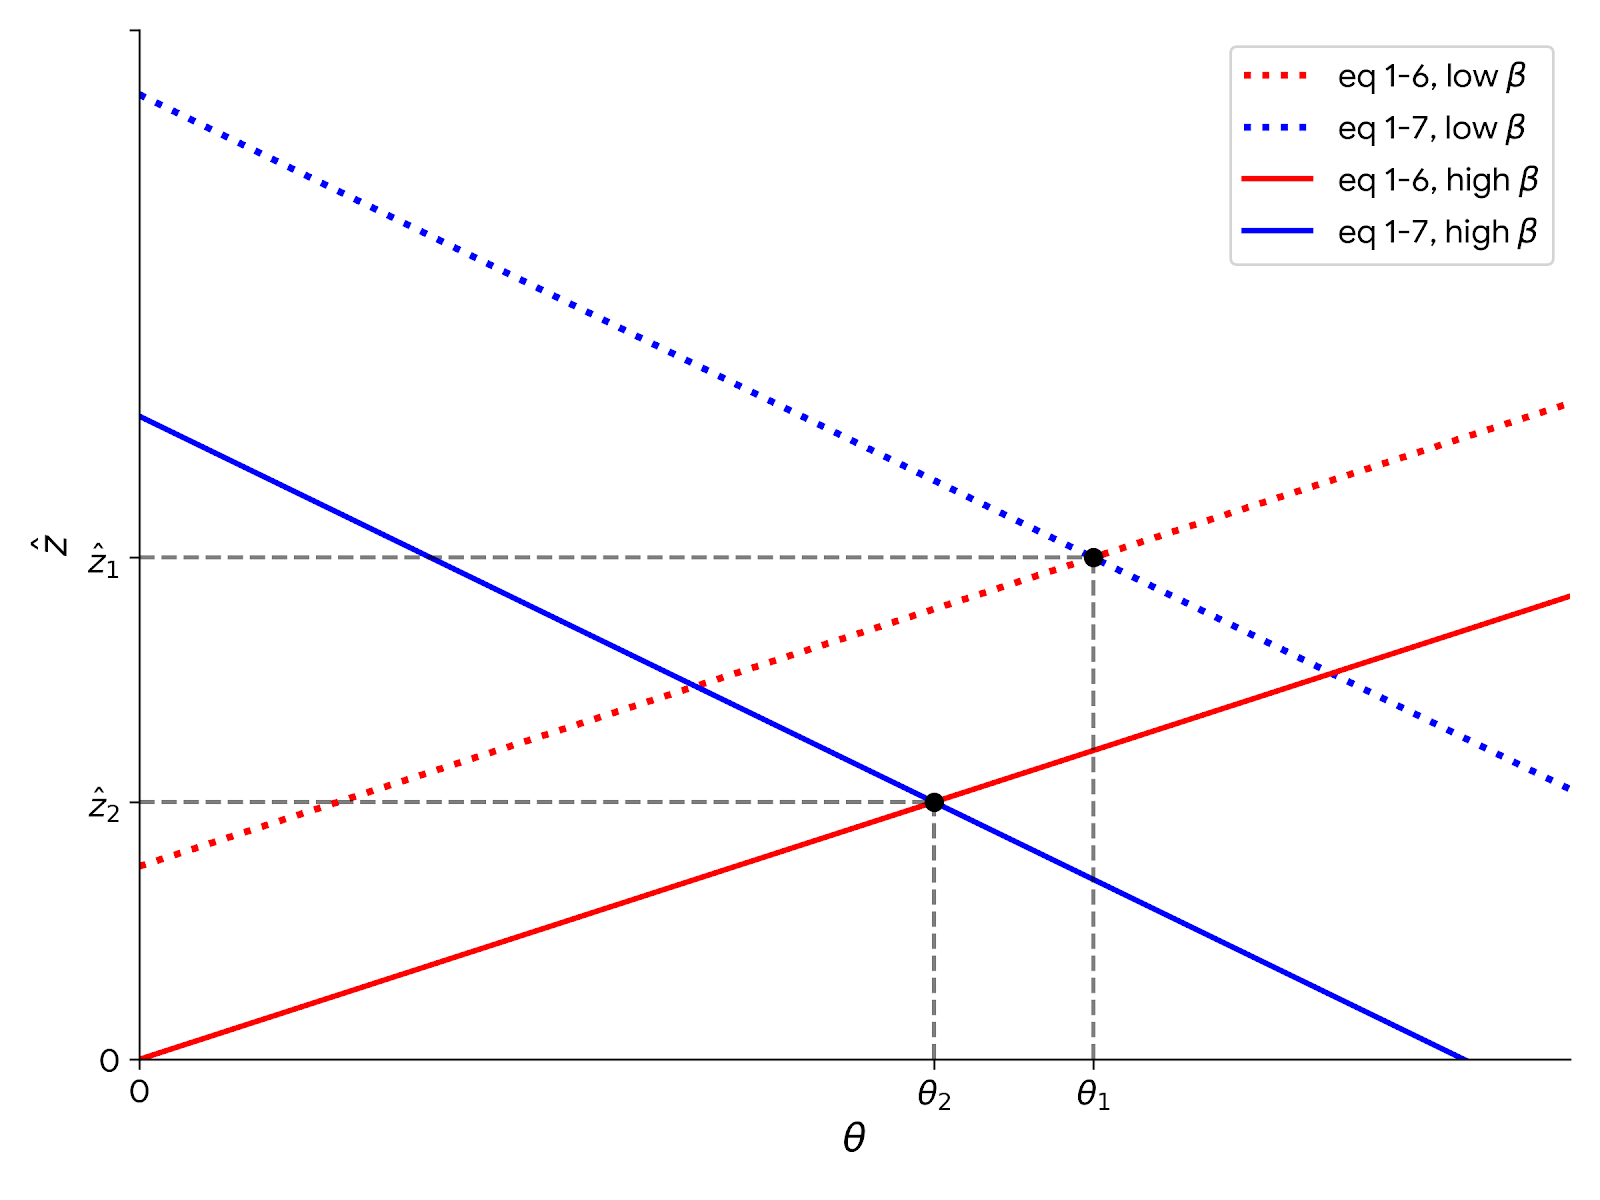
\includegraphics[width=0.65\textwidth]{Figures/q1_increase_xi.png}
  \caption{Effects of increasing $\xi$ on $\hat z$ and $\theta$}
  \label{fig:q1_increase_xi}    
\end{figure}

From above figure, a larger $\xi$ leads to a decrease in cut-off productivity $\hat z$. The effects on $\theta$ are ambiguous from the graph.\\

In each period, the productivity is realized independently of prior periods. An employed workers in period $t$ become unemployed in period $t+1$ with probability $\mathbb P(z < \hat z)$. An unemployed worker in period $t$ received a job offer with probability $f(\theta_t)$, and accepts it with probability $P(z \ge \hat z)$. Therefore, in this model, the endogenous separation rate is $s = \mathbb P(z < \hat z)$ and the endogenous job finding rate is $\tilde f = f(\theta)\mathbb P(z \ge \hat z)  $. The steady state unemployment is given by
\begin{equation*}
    \frac{u}{1-u} = \frac{s}{\tilde f} = \frac{\mathbb P(z < \hat z)}{f(\theta)\left(1-\mathbb P(z < \hat z)\right)}
\end{equation*}

When $\xi$ increases, $\hat z$ decreases and $\frac{\mathbb P(z < \hat z)}{\left(1-\mathbb P(z < \hat z)\right)}$ decreases. However, change is $f(\theta)$ depends on the distributio $G$ through equations (1-6) and (1-7), and therefore unemployment change is also dependent of distribution $G$. 

